\chapter{Ricorsione}
La programmazione ricorsiva è strettamente legata all'induzione matematica, si basa
sul fatto che per risolvere un problema mi riconduco a un problema non ancora risolto, 
ma più semplice, fino ad arrivare a un caso base già risolto.\\
I vantaggi della ricorsione sono due:
\begin{itemize}
    \item Più semplice rispetto agli algoritmi iterativi (solitamente)
    \item La logica ricorsiva è più efficiente rispetto a quella iterativa
\end{itemize}
\section{Fattoriale}
\subsection{Iterativo}
\begin{lstlisting}[language=Java]
    int Fatt(n)
        Ris=1
        For i=n downto 1
            Ris=Ris*i;
        return Ris;
\end{lstlisting}
\subsection{Ricorsivo}
\begin{lstlisting}
    int Fatt(int n)
        if n==0
            return(1);
        else
             Ris=(Fatt(n-1));
             Tot = n*Ris;
             return(Tot);
\end{lstlisting}
\section{Potenza ricorsiva}
\begin{lstlisting}{language=Java}
int Potenza (int A, int n)
c   if (n == 0)
c tif   return(1)
    else
NO c fif  Ris=A*Potenza(A, n-1)
NO c fif     return(Ris)
\end{lstlisting}
\subsection{Calcolo tempo di esecuzione}
In questo non avendo cicli dobbiamo controllare le funzioni ricorsive, è sbagliato
dire che la chiamata ricorsiva impiega $c*f_{if}$, perchè dipende da n non è un tempo
di esecuzione costante! Vedremo più avanti come calcolare il tempo di esecuzione.
\section{La ricorsione è sempre più efficiente rispetto all'iterazione?}
Prendiamo l'esempio della sequenza di Fibonacci eseguita ricorsivamente.
\begin{lstlisting}[language=Java]
int fibonacci(int n)
    if (n <= 1)
        return n;
    else 
        return fibonacci(n-1) + fibonacci(n-2);
\end{lstlisting}
Se scomponiamo l'esecuzione di questa funzione noteremo che vengono rieseguiti più volte
i calcoli per gli stessi numeri, dato che mi ritroverò più volte gli stessi numeri.
\begin{center}
    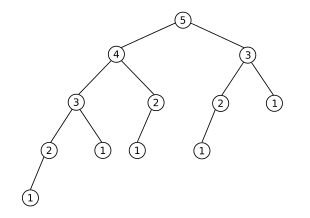
\includegraphics[width=50mm]{img/Fibonacci_Tree.png}
\end{center}
Notiamo infatti dall'albero che vengono calcolati più volte gli stessi numeri e questa
è una grande inefficienza.\\
In questi casi quindi l'iterazione risulta migliore rispetto alla ricorsione.
\section{Ricerca carattere in Array}
Dato un Array trova tutte le occorrenze di una lettera data in input (in questo caso z).\\
Devo sempre ricondurmi all'affermazione ricorsiva, quindi partire da un caso, ricondurmi
a uno più piccolo che però non mi da ancora il risultato, ma che mi avvicina sempre di più
al caso base.\\
In questo caso la penso nel seguente modo: Guarda A[n] se contiene z allora 1+tutte le z
in A[n-1] altrimenti 0 + tutte le z in A[n-1].\\
Fino a ricondurmi al primo elemento dell'array, il caso base sarà proprio quello! 
Controllare quando ho un solo elemento se è z o no, se è z ritorno 1 se no ritorno 0.
\subsection{Implementazione}
\begin{lstlisting}[language=Java]
    int trova(char car, char A[], int pos)
        if pos == 1
            if A[1] == 'z'
                return(1)
            else
                return(0)
        else
            Ris=trova(char car, char A[], pos -1)
            if A[pos] == 'z'
                Ris++
            return(Ris)
\end{lstlisting}
Solitamente nelle funzioni ricorsive per scorrere un array abbiamo bisogno di due indici,
per indicare la porzione di array che stiamo analizzando (es int h, int k), in questo
caso il primo indice è fisso dato che devo scorrere dall'ultimo valore a scendere fino al primo, quindi
sarebbe come avere h=1 fisso e k=k-1, quindi h non lo considero.\\
Le varie chiamate ricorsive mi portano a scorrere tutti i valori e quando mi riconduco al caso base, 
la risoluzione di tutte le chiamate aperte mi porta a controllare mano a mano tutti gli indici dell'array
restituendo mano a mano il contatore incrementato o meno a in base al fatto che ci sia z o meno.
        